\scanpage{193}
les $\xi_{\ell}$ du (i) dépendent du choix d'un pt géom de $X$, mais à isom non \unsure{uniques|unique} près (dépendance du \uuline{$\unsure{t_{\alpha}|{\pi}_1}(X)$}] \inserted{\figure{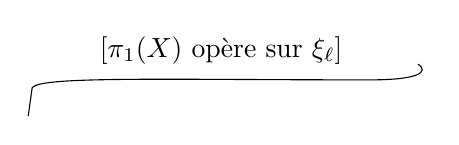
\begin{tikzpicture}[x=1cm,y=1cm]\node at (0,.35) {[$\pi_1(X)$ opère sur $\xi_\ell$]};\draw (-2.45,-.48)--(-2.4,-.12) .. controls (-2.3,.03) and (-.7,-.02) .. (1.9,-.02) .. controls (2.5,-.02) and (2.65,.08) .. (2.5,.18);\end{tikzpicture}}} sont indépendants de ce choix.

Les $\xi_p^\alpha$ dépendent du choix d'un \deleted{corps} pt \inserted{\figure{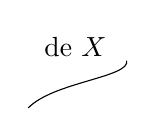
\begin{tikzpicture}[x=1cm,y=1cm]\node at (0,.35) {de $X$};\draw (-.6,-.43) .. controls (-.28,-.1) and (.7,-.04) .. (.65,.17);\end{tikzpicture}}} à valeurs dans un corps parfait sans plus, si on veut les $k(x)^{\mathrm{prf}}$\deleted{\unsure{,}} (clôture parfaite de $k(x)$), et pour $k$ donné, il ne \uline{semble pas} qu'il y ait \deleted{aie} des isom entre les $\xi_{p,a}^{(\alpha)}$ correspondant aux divers pts à valeurs dans $k$ (c'est la ``partie continue'' des $\unsure{H|H^1}$ p.ex. qui va faire des ennuis), s'ils sont localisés en le $=$ $x\in X$, \deleted{il est} \deleted{sont} si $k$ est alg. clos, ils sont conjugués par autom. de $k$ \inserted{\figure{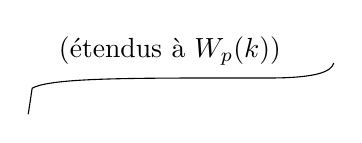
\begin{tikzpicture}[x=1cm,y=1cm]\node at (0,.35) {(étendus à $\mathbb{W}_p(k)$)};\draw (-1.8,-.45)--(-1.75,-.12) .. controls (-1.5,.02) and (-.4,.01) .. (1.25,.01) .. controls (1.9,.01) and (2.05,.1) .. (2.08,.2);\end{tikzpicture}}} les groupes alg. associés sont donc conjugués sous autom de $k$ ---- il est $=$ gentil qu'ils veuillent être l'un tordu de l'autre \ldots\ Le groupe $\pi_1(X)$ n'opère plus sur $\xi_p^\alpha$,
\margin{En revanche, on a comme structure supplémentaire les opérations $F,V$ avec $FV=p$}
par contre le groupe des autom de $k$ sur $k(x)$ \deleted{\unsure{[ou = de $k$|[ou = de $k$,}}
\deleted{\unsure{il existe]}} opère de façon $1/2$ \uline{linéaire} sur $\xi_p^{(\alpha)}$ ---- [\unsure{on|ou} a une \unsure{descente|donnée de}
\margin{élégante. D'autre part, un autom $\sigma$ de $k$ qui n'est pas $k(x)$-linéaire transforme en général $\xi_{x,p}^{\ast}$ en un $\xi_{xp}^{\sigma}$ qui n'est plus isom à $\xi_{x,p}$ ----}

Notations
\diagram{\(\begin{array}{ll}
\text{(i)}&
\left\{\begin{array}{ll}
\xi_{\bar{x},\ell} & \text{foncteur fibre $l$-adique en}\\
 & \text{le pt géom $\bar{x}$}\\
\xi_{x,\ell} & \text{par abus de langage pour $x\in X$}\\
 & \text{ou un pt de $X$ à val.}\\
 & \text{dans un corps quelc.}\\
 & \text{($\xi_{x,\ell}$ déf. à isom \uline{non unique} près)}
\end{array}\right.\\[1ex]
\text{(ii)}&
\left\{\begin{array}{ll}
\xi_{x,p}&\text{$x$ \deleted{est} pt de $X$ à val. dans un corps}\\
\xi_{x,p}^{0}&
\end{array}\right.
\end{array}\)}
\margin{\uline{On peut mettre} \uline{des exposants $\alpha$} \uline{à volonté}}
\margin{192}
